\begin{frame}
  \frametitle{DataSet}
  \begin{itemize}
  \item
    UMI-based scRNAseq Data: 5 cases vs. 5 controls
    \begin{itemize}
    \item
      In total, 26,000 cells (over 2,000 cells / individual).
    \item
      Identify cell types: using \myemph{Harmony}; choose cluster 2, which is
      cytotoxic T-cells, with 3,885 cells.
    \end{itemize}
  \item
    Select 27 genes from both top-ranked and low-ranked genes based on pseudo
    bulk analysis with \myemph{DESeq2}.
    \begin{itemize}
    \item
      Gene modules by hierarchical clustering of genes
      on cluster 2.
    \begin{itemize}
    \item
      Group1: ICAM1(DESeq2 Rank 6), XCL2 (DESeq2 Rank 13), XCL1 (DESeq2 Rank 43)
    \item
      Group2: RPS26P11 (DESeq2 Rank 15), LOC101929876 (DESeq2 Rank 22),LOC100996747 (DESeq2 Rank 97)
    \item
      Group3: HBA1 (DESeq2 Rank 14), HBA2, HBB, HBD 
    \item
      Group4: CCL3L3 (DESeq2 Rank 99), CCL3L1 (DESeq2 Rank 102), CCL3
    \end{itemize}
  \item
    Top-ranked genes: SNHG16,OASL,NAMPT,NFKB1,BCL2L11,IRF8,TPM4,TRAF4
  \item
    Low-ranked genes: KDM6A,ZNF721,HDDC2,YIPF5,MAK16, TOX
    \end{itemize}
  \end{itemize}
\end{frame}

\begin{frame}
\begin{figure}
  \centering
  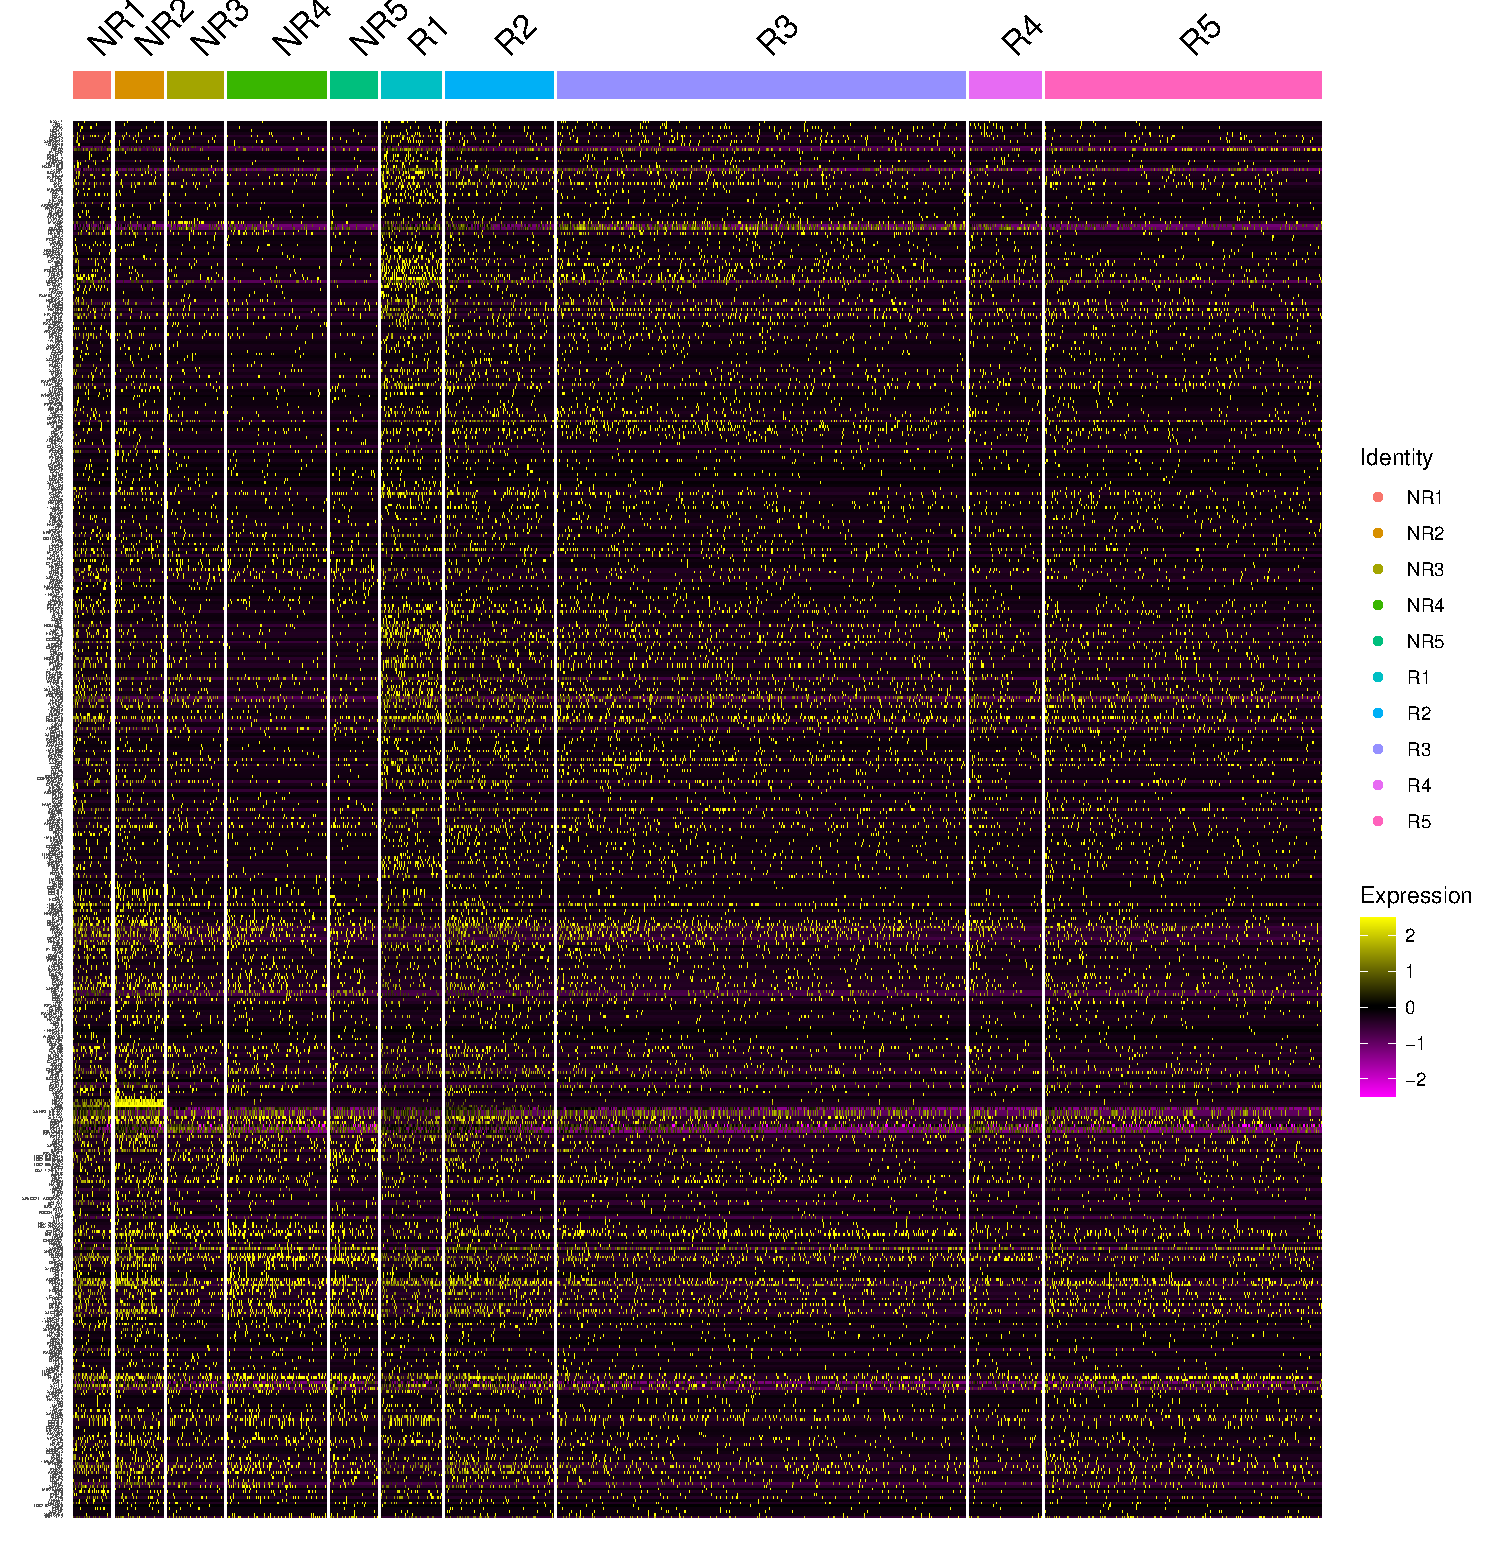
\includegraphics[height = \textheight]{gene-module-clust2.pdf}
\end{figure}
\end{frame}

\begin{frame}
  \begin{figure}
    \centering
    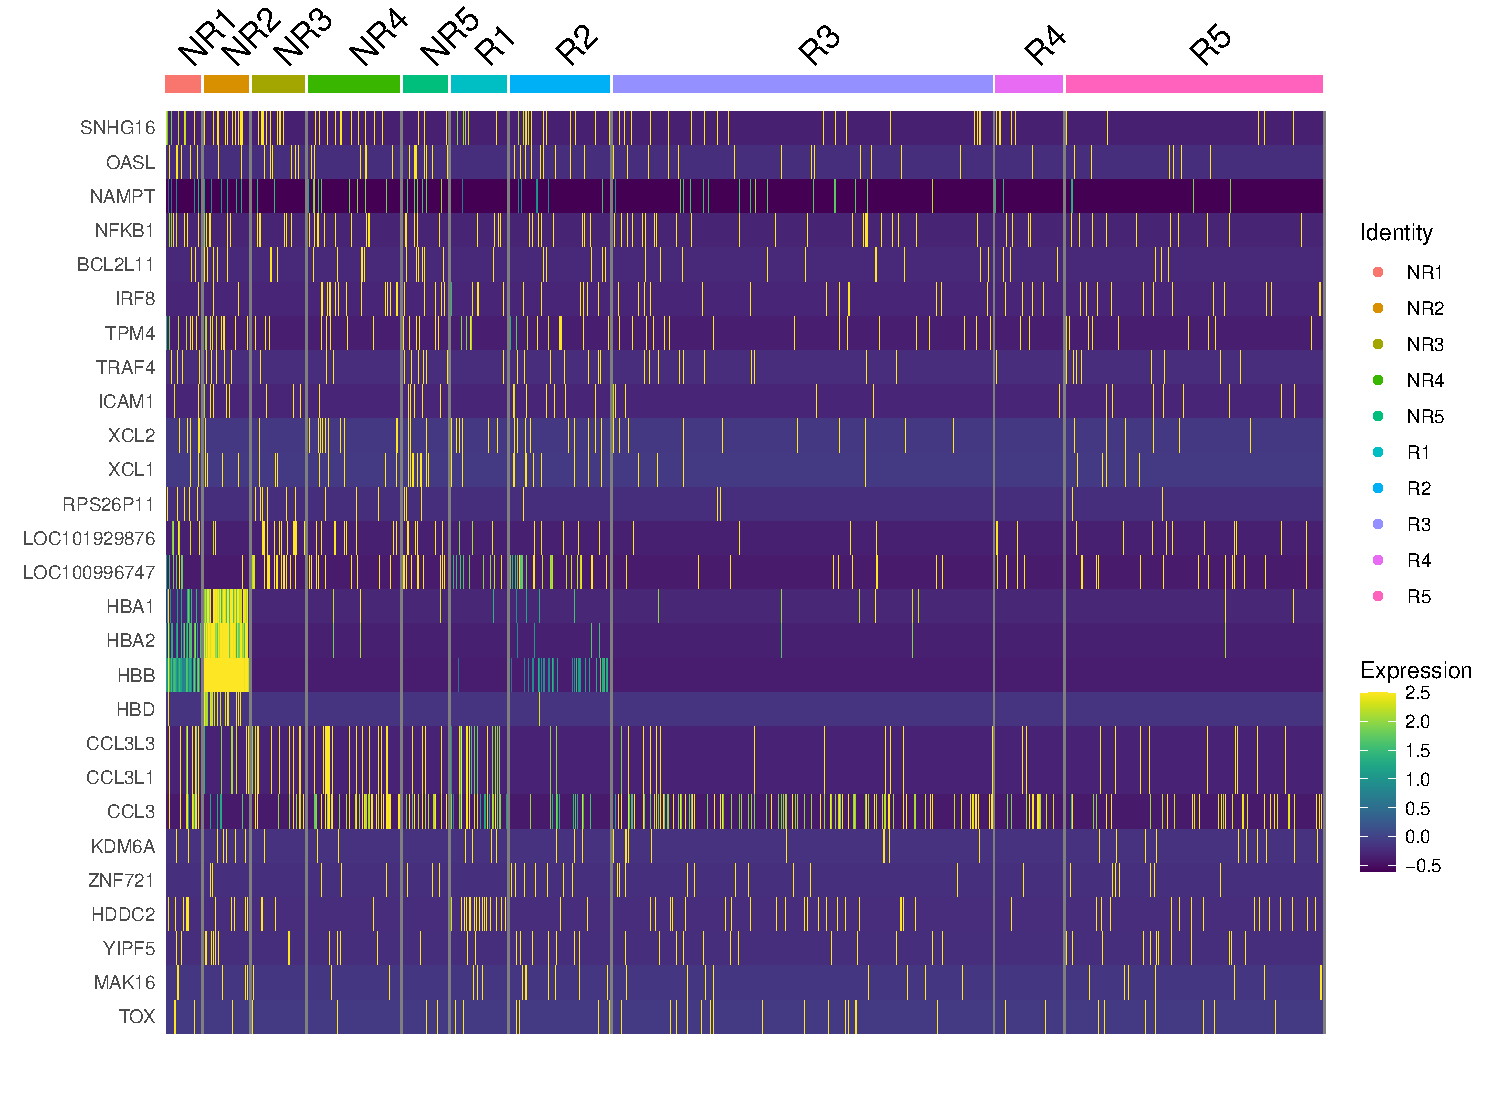
\includegraphics[width = \textwidth]{GoldGenes.pdf}
  \end{figure}
\end{frame}

\subsubsection{Gene-wise individual effect}
\begin{frame}
  \begin{figure}
    \centering
    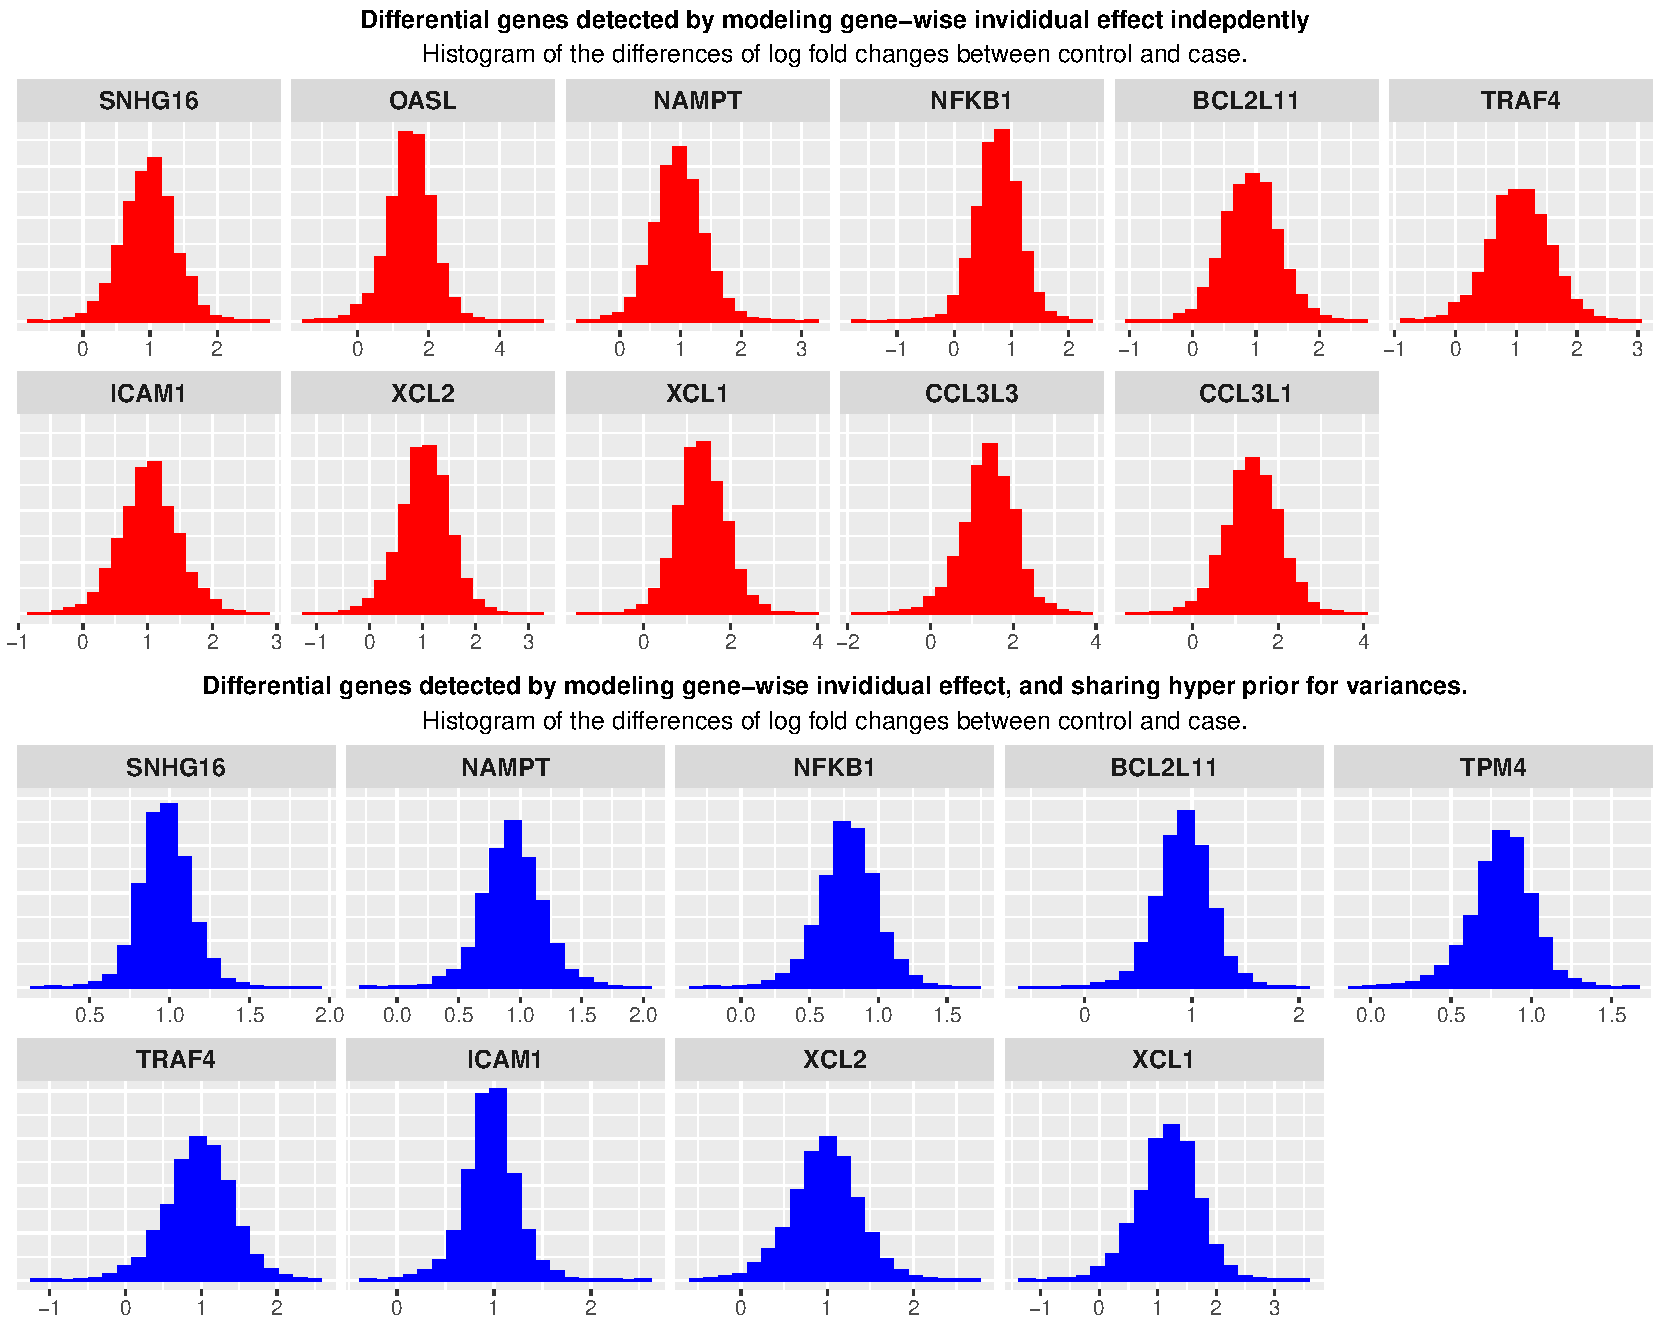
\includegraphics[height= \textheight]{v11-vs-v12-DE.pdf}
  \end{figure}
\end{frame}
\subsubsection{Gene-module individual effect}
\begin{frame}
  \begin{figure}
    \centering
    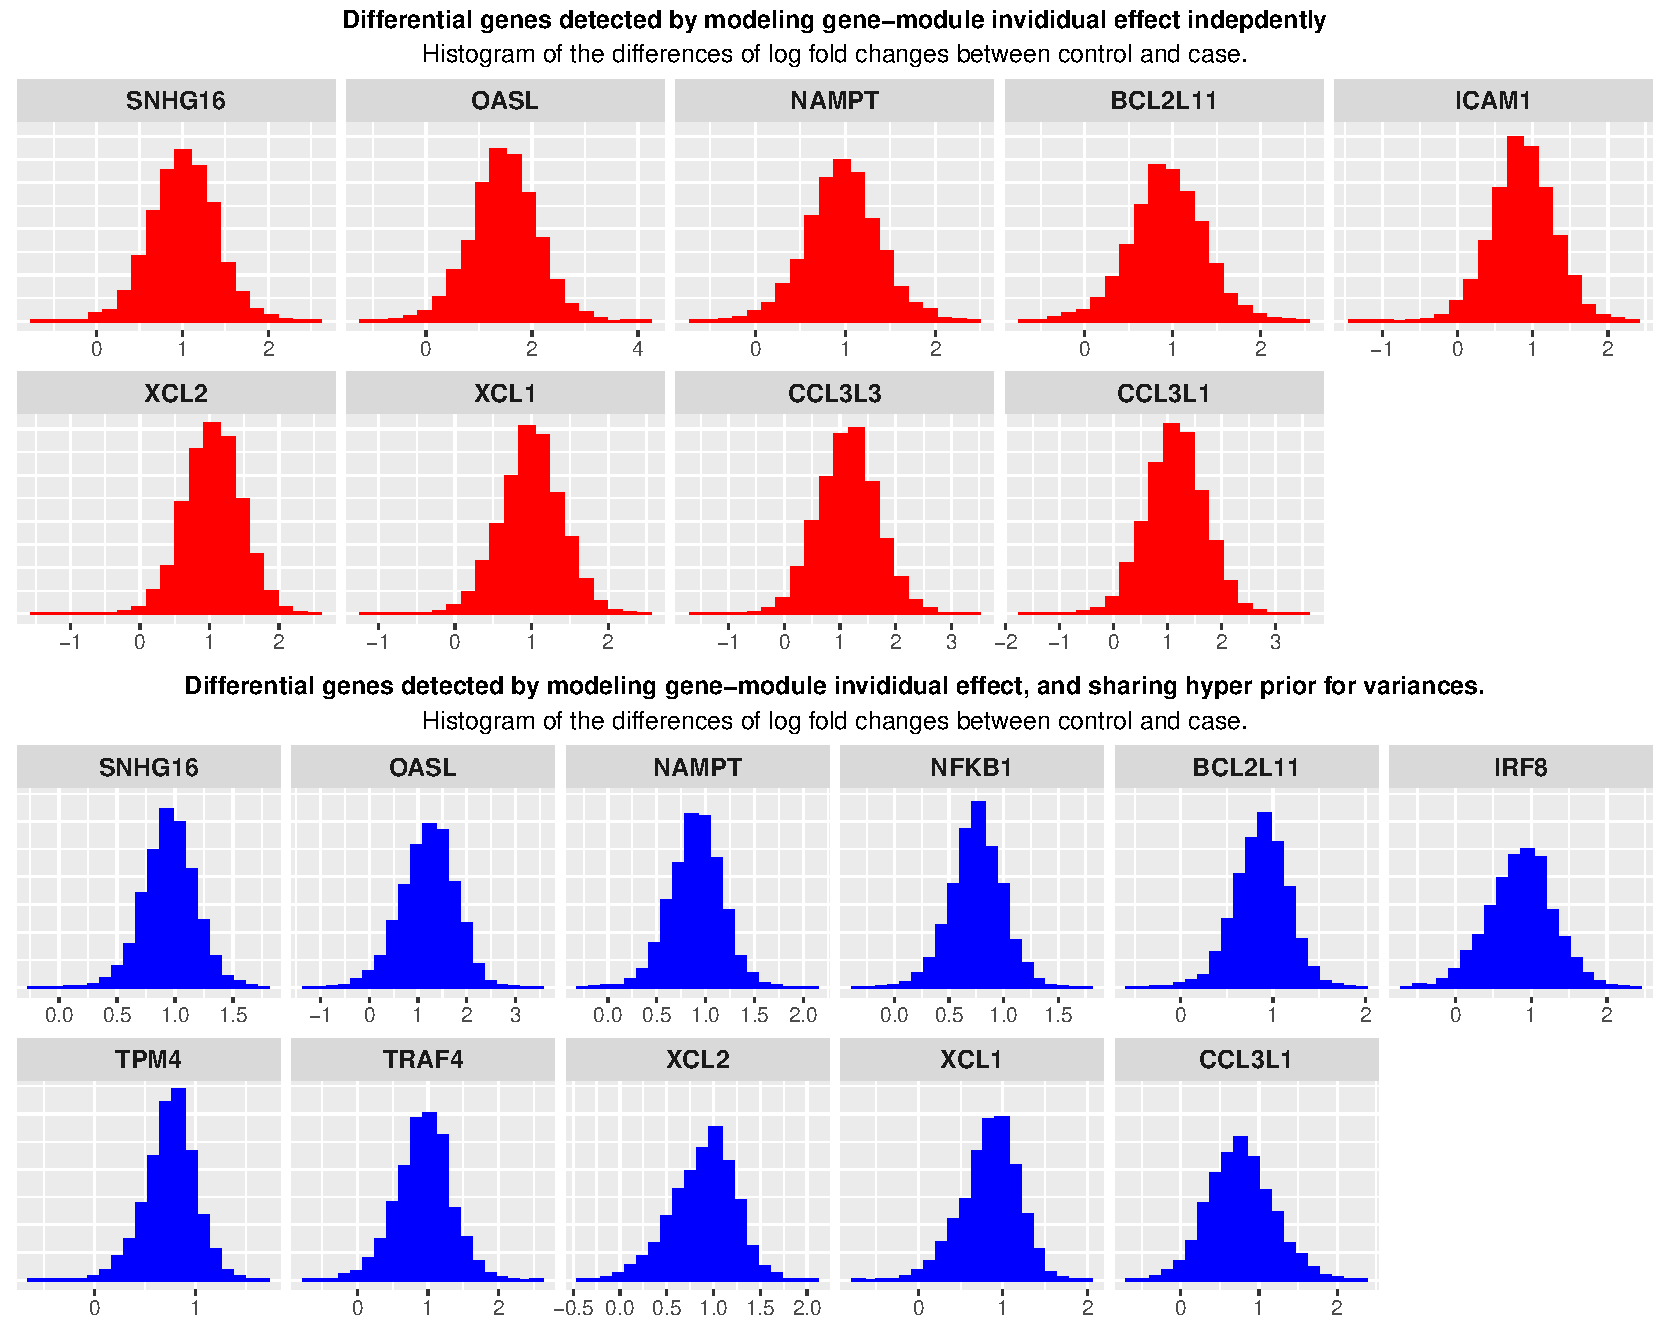
\includegraphics[height = \textheight]{v21-vs-v22-DE.pdf}
  \end{figure}
\end{frame}
